\Subhead{1.5.1}{Колебательные системы с двумя и многими степенями свободы. Нормальные колебания}
\textbf{Постановка.} Вблизи устойчивого равновесия консервативной системы кинетическая и потенциальная энергии являются квадратичными формами:
\begin{equation}
 T=\tfrac12\dot{\bm q}^{\mathsf T}M\dot{\bm q},\qquad
 U=\tfrac12{\bm q}^{\mathsf T}K\bm q,\qquad M\ddot{\bm q}+K\bm q=\bm F(t).
\end{equation}
Для обычной механической модели $M=M^{\mathsf T}>0$, $K=K^{\mathsf T}>0$. Если есть свободные симметрийные смещения, $K$ может иметь нулевые собственные значения, и соответствующие движения не являются колебаниями с ненулевой частотой. Гироскопические силы и несамосопряжённые активные связи требуют более общего анализа.

\paragraph{Собственные частоты и ортогональность.}
Подстановка $\bm q=\bm a_n\e^{-\ii\omega_nt}$ даёт
\begin{equation}\label{eq:eigenmodes}
 K\bm a_n=\omega_n^2M\bm a_n,\qquad \det(K-\omega^2M)=0.
\end{equation}
Умножим уравнения для $n$ и $m$ на $\bm a_m^{\mathsf T}$ и $\bm a_n^{\mathsf T}$ и вычтем. Симметрия $M,K$ даёт
$(\omega_n^2-\omega_m^2)\bm a_m^{\mathsf T}M\bm a_n=0$.
Различные моды ортогональны \emph{в метрике массы}. В вырожденном подпространстве можно выбрать такой же ортонормированный базис. Положим $\bm a_m^{\mathsf T}M\bm a_n=\delta_{mn}$ и разложим
\begin{equation}
 \bm q(t)=\sum_n\bm a_nQ_n(t),\quad
 \ddot Q_n+\omega_n^2Q_n=F_n(t),\quad F_n=\bm a_n^{\mathsf T}\bm F.
\end{equation}
Нормальная мода --- согласованное движение всех координат с одной частотой и неизменными отношениями амплитуд. Нормальная координата описывает возбуждение этой моды, а не смещение отдельной части системы.

\paragraph{Два связанных осциллятора и биения.}
Для двух одинаковых масс $m$, собственных пружин $k$ и связующей пружины $k_c$:
\begin{equation}
 M=m\begin{pmatrix}1&0\\0&1\end{pmatrix},\quad
 K=\begin{pmatrix}k+k_c&-k_c\\-k_c&k+k_c\end{pmatrix},\quad
 \omega_{\mathrm s}=\sqrt{k/m},\quad
 \omega_{\mathrm a}=\sqrt{(k+2k_c)/m}.
\end{equation}
Симметричная мода имеет $q_1=q_2$, антисимметричная $q_1=-q_2$. При $q_1(0)=A$, $q_2(0)=0$, нулевых скоростях
\begin{align}
 q_1&=\tfrac A2(\cos\omega_{\mathrm s}t+\cos\omega_{\mathrm a}t)
 =A\cos\bar\omega t\cos\tfrac{\Delta\omega t}{2},\\
 q_2&=\tfrac A2(\cos\omega_{\mathrm s}t-\cos\omega_{\mathrm a}t)
 =A\sin\bar\omega t\sin\tfrac{\Delta\omega t}{2},
\end{align}
где $\Delta\omega=\omega_{\mathrm a}-\omega_{\mathrm s}$ и $\bar\omega=(\omega_{\mathrm a}+\omega_{\mathrm s})/2$. При слабой связи наблюдается медленный обмен энергией с периодом $2\pi/\Delta\omega$. Это биения двух независимых нормальных мод, а не самопроизвольное изменение их собственных частот.

\paragraph{Парциальные частоты.}
В записи $\ddot x_1+\omega_a^2x_1=gx_2$, $\ddot x_2+\omega_b^2x_2=gx_1$ величины $\omega_a,\omega_b$ --- частоты при закреплении другой подсистемы, $[g]={\rm с}^{-2}$. Нормальные частоты всей системы:
\begin{equation}\label{eq:avoidedcrossing}
 \omega_\pm^2=\frac{\omega_a^2+\omega_b^2}{2}
 \pm\sqrt{\left(\frac{\omega_a^2-\omega_b^2}{2}\right)^2+g^2}.
\end{equation}
При положительно определённой жёсткости обе частоты вещественны. Связь раздвигает их относительно парциальных; при перестройке наблюдается избегаемое пересечение. Знак $g$ меняет формы мод, но не эти частоты.
\begin{center}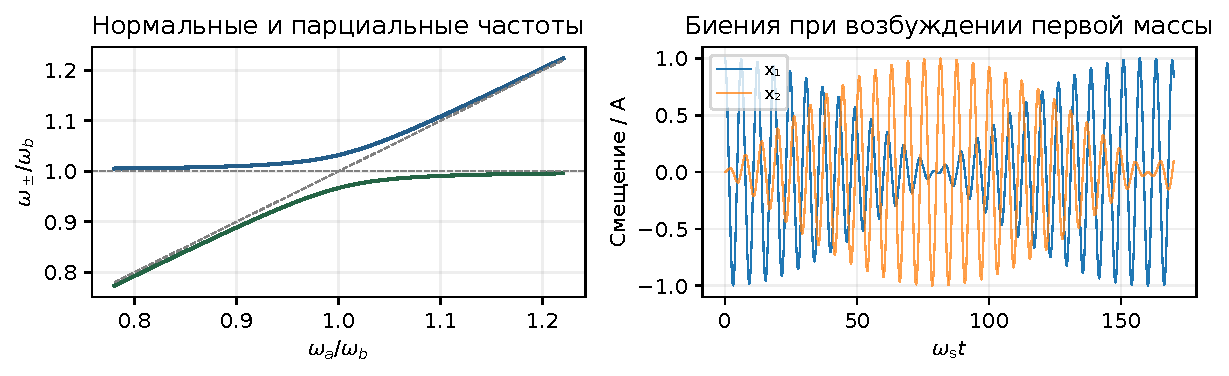
\includegraphics[width=.83\linewidth]{figures/coupled_modes.pdf}\end{center}
% Альтернативное объяснение: вопрос 5 коллеги начинает с x1+x2 и x1-x2.
% Здесь сохранена предпочтенная В. матричная постановка; пример показывает тот же результат.
